\subsection{Scale-Invariant Feature Transform (SIFT)}
Das folgende Kapitel basiert auf David G. Lowes Paper ''Distinctive Image Features
from Scale-Invariant Keypoints'' \footnote{\cite{Lowe2004}}

In seinem Paper ''Distinctive Image Features from Scale-Invariant Keypoints'' von 2004 stellte David G. Lowe eine Methode zur Merkmalsfindung und Merkmalsbeschreibung vor.

Das Verfahren wurde mit dem Ziel entworfen, dass Merkmale unabhängig von Rotation und Skalierung gefunden werden. So sollen Objekte in Bildern wiedergefunden werden können, wenn sie gedreht oder näher bzw. weiter weg sind.

Die SIFT Merkmale werden in 4 Schritten berechnet.

\begin{enumerate}

\item Extrema im Skalenraum finden, die potentielle Keypoints sein können
\item Prüfen, ob die zuvor gefundenen Punkte geeignete Keypoints sind
\item Zuweisen einer Orientierung für den Bildausschnitt
\item Erstellen des Deskriptors

\end{enumerate}

\subsubsection{Merkmalserkennung}

Da SIFT versucht Merkmale zu finden, die für verschiedene Skalierungen des Bildes konstant sind, müssen Punkte gefunden werden, die invariant zur Skalierung des Bildes sind.
Für die Erkennung von Merkmalen soll sich also nicht auf Details, die in höheren Skalierungen verloren gehen verlassen, sondern Punkte gefunden werden, die im Skalenraum Extrema sind.

Es wurde von Lowe gezeigt \footnote{\cite{Lowe:1999:ORL:850924.851523}}, dass Merkmale im Skalenraum durch Extrema der Differenz der Gauß Funktionen gefunden werden können.
Sei $I(x, y)$ das Bild, $G(x, y, \sigma)$ die zwei Dimensionale Gaußfunktion  und $L(x, y, \sigma)$ die Skalenraumfunktion.
Die Differenz der Gaußfunktionen $D(x, y, \sigma)$ für zwei Skalierungen, die um einen Faktor $k$ im Skalenraum entfernt sind, ist definiert als:

\[
D(x, y, \sigma) = G(x, y, k\sigma) - G(x, y, \sigma)) * I(x, y)\\ = L(x, y, k\sigma) - L(x, y, \sigma)
\]

Die Differenz der Gaußfunktionen zeigt, welche Strukturen in dem Übergang von einer Skalierung in die andere verloren gehen. In Abbildung \ref{fig:dogSample} ist dies für das Bild aus Abbildung \ref{fig:scaleSpace} dargestellt.

\begin{figure}[h]
    \centering
		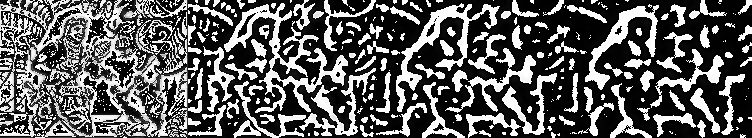
\includegraphics[scale=0.55]{bilder/firstDiv.png}
    	\caption{Differenz der Gaußfunktionen aus Abbildung \ref{fig:scaleSpace}. Die weißen Bereiche zeigen die Bereiche an, in denen Details verloren gehen.}

\label{fig:dogSample}
\end{figure}


Um die Differenz der Gaußfunktionen effizient zu berechnen, wird das Eingabebild mehrmals mit der Gaußfunktion gefaltet, um mehrere Skalierungen des Bildes zu erzeugen. Die einzelnen Skalierungen liegen immer um den Faktor $k$ auseinander.  Es werden jeweils von 2 Skalierungen, die im Skalenraum nebeneinander sind, die Differenz gebildet.
Sobald eine Oktave im Skalenraum durchlaufen ist, wird die Auflösung des Ursprungsbildes der Oktave halbiert. Dieses Bild bildet den Anfang der nächsten Oktave.
Dieser Vorgang wird in Abbildung \ref{fig:siftDog} dargestellt.

\begin{figure}[h]
    \centering
		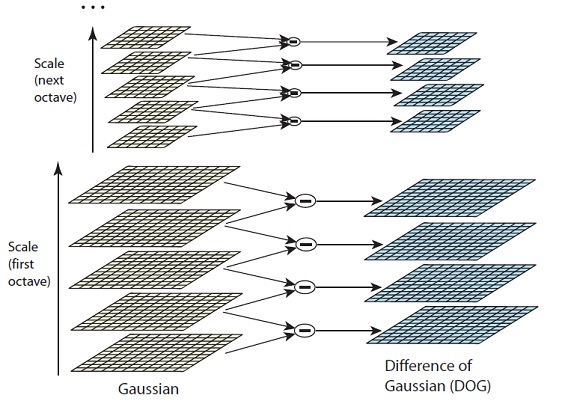
\includegraphics[scale=0.8]{bilder/sift-dog-idea.jpg}
    	\caption{Differenz der Gaußfunktionen für verschiedene Skalierungen und Oktaven (Abbildung aus \cite[S. 6]{Lowe2004}).}
\label{fig:siftDog}
\end{figure}

Um nun lokale Extrema im Scale Space zu finden, werden viele Beispielpunkte aus verschiedenen Skalierungen und Oktaven gewählt. Es werden drei Skalierungen pro Oktave betrachtet. Die Oktaven werden weitergeführt, bis die Bildauflösung zu gering ist.

Für jeden Punkt wird nun überprüft, ob er ein lokales Extremum ist. Dafür wird geprüft, ob der Punkt größer oder kleiner als alle seine Nachbarn in seiner eigenen Skalierung und in den Skalierungen darüber und darunter ist.

\begin{figure}[h]
    \centering
		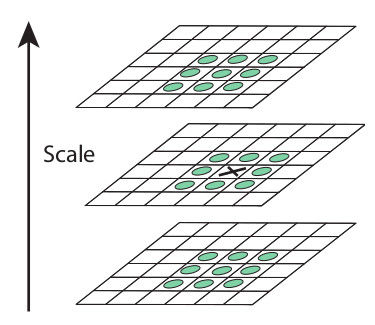
\includegraphics[scale=0.4]{bilder/sift_extrema.png}
    	\caption{Um ein Extremum zu sein, muss der mit X markierte Punkt größer oder kleiner sein als alle Nachbarn in anliegenden Scales (Abbildung aus\cite[S. 7]{Lowe2004}).}
\end{figure}

Viele der so gefunden Punkte sind nicht geeignet um stabile Merkmale zu sein:

Punkte mit zu geringem Kontrast (\ref{sec:kontrast}) sind nicht robust gegenüber Bildrauschen (\ref{sec:rauschen}). Durch den geringen Kontrast kann bereits leichtes Bildrauschen den Bereich stark verfälschen.
Deshalb werden von den potentiellen Merkmalen alle Punkte, deren Umgebung einen zu geringen Kontrast aufweist, entfernt.

Wie in \ref{sec:featureDetection} erwähnt, lassen sich Punkte entlang Kanten nicht gut an der Kante lokalisieren.

Der Gradient an Punkte, die an einer Kante liegen, ist in die Richtung der Kante sehr gering und in die Richtung entgegen der Kante sehr groß. Bei einer Ecke hingegen sind die Gradienten in alle Richtungen groß.
Für den Punkt wird die Richtung mit dem größten Gradienten gesucht und die Richtung rechtwinkling zu dieser. Ist das Verhältnis der Gradienten in die beiden Richtungen groß, so liegt der Punkt an einer Kante.

Um Punkte entlang Kanten zu entfernen, wird die Krümmung an dem jeweiligen Punkt betrachtet. Als Krümmung wird in diesem Zusammenhang die Ableitung der Gradiente verstanden. Die Richtung, in die die Krümmung am stärksten ist, wird als Hauptkrümmung bezeichnet.
Eine Kante hat eine starke Krümmung rechtwinklig zur Kante. Jedoch ist die Krümmung in Richtung der Kante sehr klein. 
Es wird nun das Verhältnis der Hauptkrümmung und der Krümmung rechtwickling zur Hauptkrümmung betrachtet.
Bei einer Ecke sind beide Krümmungen groß, also der Quotient der beiden gering. Bei einer Kante ist nur die Hauptkrümmung groß. Dadurch ist auch der Quotient groß. 
Ist das Verhältnis der beiden Krümmungen zu groß, wird der Punkt nicht mehr weiter betrachtet.


Die übrig gebliebenen Punkte werden nun Orientierungen zugewiesen und verwendet, um Merkmale zu bilden.


Um einem Punkt eine Orientierung zuzuweisen, wird für eine Region um ihn die Richtung $\theta(x, y)$ und Größe $m(x, y)$ der Gradienten berechnet. Das $\sigma$ entspricht der Skalierung, in der der Punkt gefunden wurde.
\[
m(x, y) = \sqrt{(L(x + 1, y, \sigma) - L(x - 1, y, \sigma))^2 + (L(x, y + 1, \sigma) - L(x, y - 1, \sigma))^2}
\]

\[
\theta(x, y)) = \tanh^{-1}((L(x + 1, y, \sigma) - L(x - 1, y, \sigma)) / (L(x, y + 1, \sigma) - L(x, y - 1, \sigma)))
\]

Es wird nun ein Histogramm der Gradientenrichtungen gebildet. Dieses Histogramm hat 36 Klassen, die jeweils 10° abdecken. Bei jedem hinzugefügten Punkt aus der Region wird dieser mit dem Gewicht $m(x, y)$ und einer Gaußgewichtung um den Ursprungspunkt des Ausschnittes gewichtet.
Aus dem Histogramm können nun durch die Spitzen die Orientierung der Region abgelesen werden. Sollte eine weitere Spitze nicht kleiner als 80\% der größten Spitze sein, wird für diese auch ein Merkmal erstellt. So enstehen für Regionen mit mehren Hochpunkten im Richtungshistogramm auch mehrere Merkmale.

\subsubsection{Merkmalsbeschreibung}

Nachdem einem Bildausschnitt eine Skalierung und eine Orientierung zugeordnet wurde, wird in diesem Schritt eine vektorielle Darstellung von diesem Aussschnit erstellt.


Der Deskriptor wird für eine $16 \times 16$ Umgebung um den Punkt gebildet. Hierbei wird für jeden Pixel in der Umgebung die Richtung $\theta(x, y)$ und Stärke $m(x, y)$ des Gradienten berechnet. Die Richtung wird um die zuvor gefundene Rotation gedreht, damit eine Unabhängigkeit von der Rotation gegeben ist.

Die Gradienten werden mit einem Gaußfenster gewichtet und in $4 \times 4$ Regionen eingeteilt (siehe Abbildung \ref{fig:siftDesc}). In diesen Regionen werden die Gradienten einer von 8 Richtungen zugeordnet, der sie am nächsten sind. Damit bildet jede Region einen 8 dimensionalen Merkmalsvektor. Der enstehende Deskriptor für den Bildausschnitt ist somit $4 \times 4 \times 8$.



\begin{figure}[h]
    \centering
		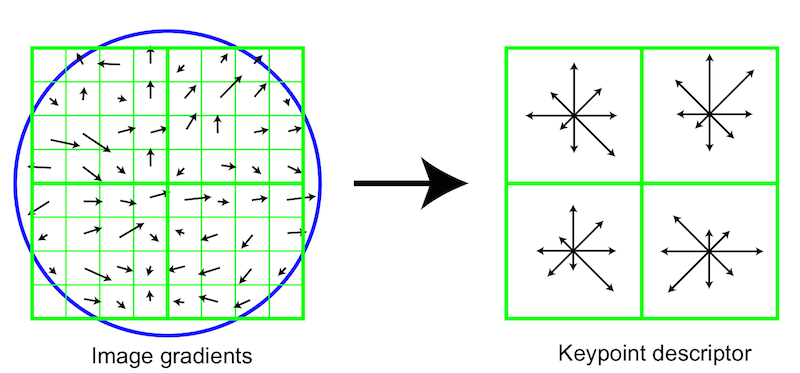
\includegraphics[scale=0.8]{bilder/sift_pic.png}
    	\caption{Umwandlung der Gradienten in den Descriptor für einen $8 \times 8$ Bildausschnitt. SIFT benutzt einen $16 \times 16$ Ausschnitt, aus dem ein $4 \times 4$ Descriptor erstellt wird.  Der blaue Kreis stellt die Gaußgewichtung dar (Abbildung aus\cite[S. 15]{Lowe2004}).}
 \label{fig:siftDesc}
\end{figure}

